\documentclass[10pt,twocolumn,3p,times]{article}

% --- Packages ---
\usepackage[utf8]{inputenc}
\usepackage[margin=0.75in]{geometry}
\usepackage{amsmath,amssymb,amsfonts,amsthm}
\usepackage{booktabs}
\usepackage{cite}
\usepackage{microtype}
\usepackage{graphicx}
\usepackage{subcaption}
\usepackage{xcolor}
\usepackage{url}
\usepackage{hyperref}
\usepackage{tikz}
\usetikzlibrary{shapes.geometric, arrows.meta, positioning, fit, backgrounds, calc}

% --- Color Definitions ---
\definecolor{primaryblue}{RGB}{20, 50, 120}
\definecolor{secondaryteal}{RGB}{0, 130, 140}
\definecolor{accentdark}{RGB}{40, 40, 50}
\definecolor{boxbg}{RGB}{245, 247, 250}

% --- Hyperref Setup ---
\hypersetup{
    colorlinks=true,
    linkcolor=primaryblue,
    citecolor=primaryblue,
    urlcolor=secondaryteal,
    pdftitle={HypothesisOS: Compute-Efficient Autonomous ML Discovery via Multi-Agent Deliberation and State-Tree Search},
    pdfauthor={Assem El-Qersh}
}

% --- TikZ Style Definitions ---
\tikzstyle{block} = [rectangle, draw=primaryblue, fill=boxbg, thick, minimum width=2.2cm, minimum height=1.0cm, align=center, rounded corners=3pt, font=\small]
\tikzstyle{process} = [rectangle, draw=secondaryteal, fill=boxbg, thick, minimum width=2.0cm, minimum height=0.9cm, align=center, rounded corners=2pt, font=\small]
\tikzstyle{decision} = [diamond, draw=primaryblue, fill=boxbg, thick, minimum width=1.5cm, minimum height=1.0cm, align=center, font=\scriptsize]
\tikzstyle{line} = [draw, -{Stealth[length=2.5mm]}, thick, primaryblue]
\tikzstyle{dashedline} = [draw, -{Stealth[length=2.5mm]}, dashed, thick, secondaryteal]

\title{\textbf{\Large HypothesisOS: Compute-Efficient Autonomous ML Discovery via Multi-Agent Deliberation and State-Tree Search}}

\author{
    \textbf{Assem El-Qersh}\\[0.5em]
    \small Department of Computer Science / Independent Research\\
    \small \href{mailto:assem.elqersh@gmail.com}{\texttt{assem.elqersh@gmail.com}}
}

\date{\small October 2026}

\begin{document}

\maketitle

\begin{abstract}
Autonomous machine learning (ML) discovery systems have emerged as a promising frontier, automating iterative code mutation, training, and evaluation. However, existing frameworks suffer from critical efficiency bottlenecks: greedy linear exploration, self-preference biases in single-agent evaluators, uncalibrated utility estimations, and uncontrolled compute consumption. In this paper, we present \textbf{HypothesisOS}, a compute-normalized experiment controller designed to maximize validated scientific progress per unit GPU-hour and LLM token cost. HypothesisOS integrates a multi-hypothesis proposal generator, an anonymized multi-LLM review council utilizing Kendall's $W$ concordance and mean-rank aggregation, a cost-aware Expected Value (EV) acquisition function, and a state-tree Upper Confidence bounds applied to Trees (UCT) search algorithm with recursive value backpropagation and branch-isolated code restoration. We formalize the research objective as compute-normalized validation improvement, present an exhaustive 7-armed factorial ablation protocol across standardized benchmarks, and specify an integrity-checked evaluation boundary that prevents validation data leakage. Our theoretical and empirical analysis demonstrates that cost-aware multi-agent experiment control systematically outperforms greedy single-agent baselines in discovery yield per unit compute.
\end{abstract}

\textbf{\small Keywords:} Autonomous Machine Learning, Multi-Agent Systems, Experiment Controller, Upper Confidence Bounds on Trees (UCT), Expected Value Acquisition, Compute-Normalized Discovery.

\section{Introduction}
\label{sec:intro}

The automation of machine learning research has transitioned from brute-force hyperparameter optimization to agentic systems capable of modifying source code, executing empirical training loops, and interpreting quantitative results~\cite{karpathy2026autoresearch, lu2024aiscientist}. Recent breakthroughs such as Karpathy's \textit{AutoResearch}~\cite{karpathy2026autoresearch}, Sakana AI's \textit{The AI Scientist v2}~\cite{lu2025aiscientistv2}, and EvoScientist~\cite{lu2026evoscientist} demonstrate that Large Language Models (LLMs) can autonomously discover novel neural architectures and training schedules.

Despite these advancements, current autonomous research platforms exhibit key architectural vulnerabilities:
\begin{enumerate}
    \item \textbf{Greedy Linear Search Collapse:} Single-agent frameworks iterate sequentially along a single code lineage, abandoning promising alternative branches whenever a trial fails.
    \item \textbf{Evaluator Self-Preference Bias:} Single LLM evaluators frequently suffer from self-grading bias, favoring their own generation style or output patterns over objective merit.
    \item \textbf{Unconstrained Compute Consumption:} Existing architectures optimize raw performance without explicitly modeling the trade-off between expected validation gain, information surprise, and execution cost (GPU wall-clock time and LLM token usage).
    \item \textbf{State Contamination \& Evaluator Leakage:} Mutating working code without isolated state snapshots leads to cross-branch contamination, while unshielded evaluation scripts allow patches to tamper with validation metrics or dataset splits.
\end{enumerate}

To resolve these failure modes, we introduce \textbf{HypothesisOS}, an empirical systems framework and compute-normalized experiment controller. HypothesisOS shifts the paradigm from unconstrained code generation to principled experiment control.

\subsection{Formal Objective Function}

We formalize autonomous ML discovery as an optimization problem under finite resource constraints. Let $\Delta_{\text{val}}$ denote the empirical reduction in validation metric (e.g., bits-per-byte, BPB) achieved by an experimental code patch over its parent state. Let $t_{\text{GPU}}$ represent the execution wall-clock GPU hours, and $T_{\text{LLM}}$ denote total LLM token consumption converted to GPU-equivalent cost via scalar $c_{\text{LLM}}$.

The overall objective of the HypothesisOS controller is to maximize the compute-normalized discovery rate $\mathcal{E}$:
\begin{equation}
    \mathcal{E} = \frac{\mathbb{E}[\Delta_{\text{val}}]}{\text{GPU-hours} + c_{\text{LLM}} \cdot T_{\text{LLM}}}
    \label{eq:objective}
\end{equation}
subject to total budget constraints $B_{\text{GPU}}$ and $B_{\text{token}}$.

\section{Survey of Prior Art}
\label{sec:prior_art}

HypothesisOS builds upon foundational contributions in AutoML, neural architecture search (NAS), multi-agent deliberation, and tree-structured hypothesis exploration (2023--2026). Table~\ref{tab:prior_art_comparison} provides an exhaustive comparative analysis across existing autonomous research frameworks.

\begin{table*}[t]
\centering
\caption{Systematic comparison of modern autonomous ML research systems and experiment controllers (2023--2026).}
\label{tab:prior_art_comparison}
\small
\resizebox{\textwidth}{!}{%
\begin{tabular}{l l l l l l}
\toprule
\textbf{System / Framework} & \textbf{Agent Architecture} & \textbf{Search Structure} & \textbf{Memory \& State Tracking} & \textbf{Evaluation \& Security} & \textbf{Primary Innovation / Limitation} \\
\midrule
\textbf{AutoResearch}~\cite{karpathy2026autoresearch} & Single LLM Agent & Linear Chain (Keep/Revert) & Git Working Directory & Metric threshold (\texttt{val\_bpb}) & Minimal 630-line loop; lacks branching/council. \\
\textbf{LLM Council}~\cite{karpathy2025llmcouncil} & Anonymized Committee & Parallel Consensus & Session Context & Mean-Rank Voting & Eliminates self-bias; no training loop execution. \\
\textbf{AI Scientist v2}~\cite{lu2025aiscientistv2} & Multi-Agent Team & Agentic Tree Search & Dynamic Experiment Tree & Simulated Reviewer Loop & First AI paper submission; high compute footprint. \\
\textbf{EvoScientist}~\cite{lu2026evoscientist} & 3 Specialized Agents & Evolutionary Search & Ideation \& Experiment Memory & Code Success \& Novelty & Avoids failure repetition; heuristic search rule. \\
\textbf{AutoDiscovery}~\cite{autodiscovery2025} & Bayesian LLM Gen. & MCTS with Surprise Reward & Local Search Tree & Bayesian Surprisal Metric & Open-ended discovery; lacks compute-cost term. \\
\textbf{Consensus NAS}~\cite{consensusnas2026} & 3--5 Debating LLMs & Consensus NAS Debate & Single-shot State & Validation Metric (F1) & Discrete architecture NAS; no long-term tree. \\
\textbf{AlphaEvolve}~\cite{alphaevolve2025} & Evolutionary LLM Pool & Program Population & Population Buffer & Automated Task Verification & Discovered 4$\times$4 matrix mult.; domain specific. \\
\midrule
\textbf{HypothesisOS} (\textbf{Ours}) & \textbf{Anonymized Council} & \textbf{State-Tree UCT} & \textbf{Snapshot State DAG} & \textbf{SHA-256 Hash Lock + Isolated} & \textbf{Compute-normalized EV acquisition \& UCT backprop.} \\
\bottomrule
\end{tabular}%
}
\end{table*}

Key developments informing our architecture include:
\begin{itemize}
    \item \textbf{AutoResearch}~\cite{karpathy2026autoresearch}: Established single-file \texttt{train.py} modification loops with automatic git rollback, proving that minimal standardized execution cycles generate compounding gains.
    \item \textbf{LLM Council}~\cite{karpathy2025llmcouncil}: Introduced anonymized multi-model peer review, demonstrating that masking model identities eliminates self-preference bias during proposal selection.
    \item \textbf{AI Scientist v2}~\cite{lu2025aiscientistv2}: Extended discovery to progressive agentic tree search, enabling branching exploration of sub-experiments.
    \item \textbf{EvoScientist}~\cite{lu2026evoscientist}: Demonstrated the necessity of persistent ideation and failure memory modules to prevent redundant experiments.
\end{itemize}

\section{System Architecture \& Methodology}
\label{sec:architecture}

HypothesisOS is organized into five decoupled layers: (1)~Proposal Engine, (2)~Anonymized Multi-LLM Review Council, (3)~Cost-Aware Acquisition Engine, (4)~State-Tree UCT Search Navigator, and (5)~Sandboxed Execution Layer with an Integrity-Checked Evaluator. Figure~\ref{fig:tikz_architecture} illustrates the systematic data flow.

\begin{figure*}[t]
\centering
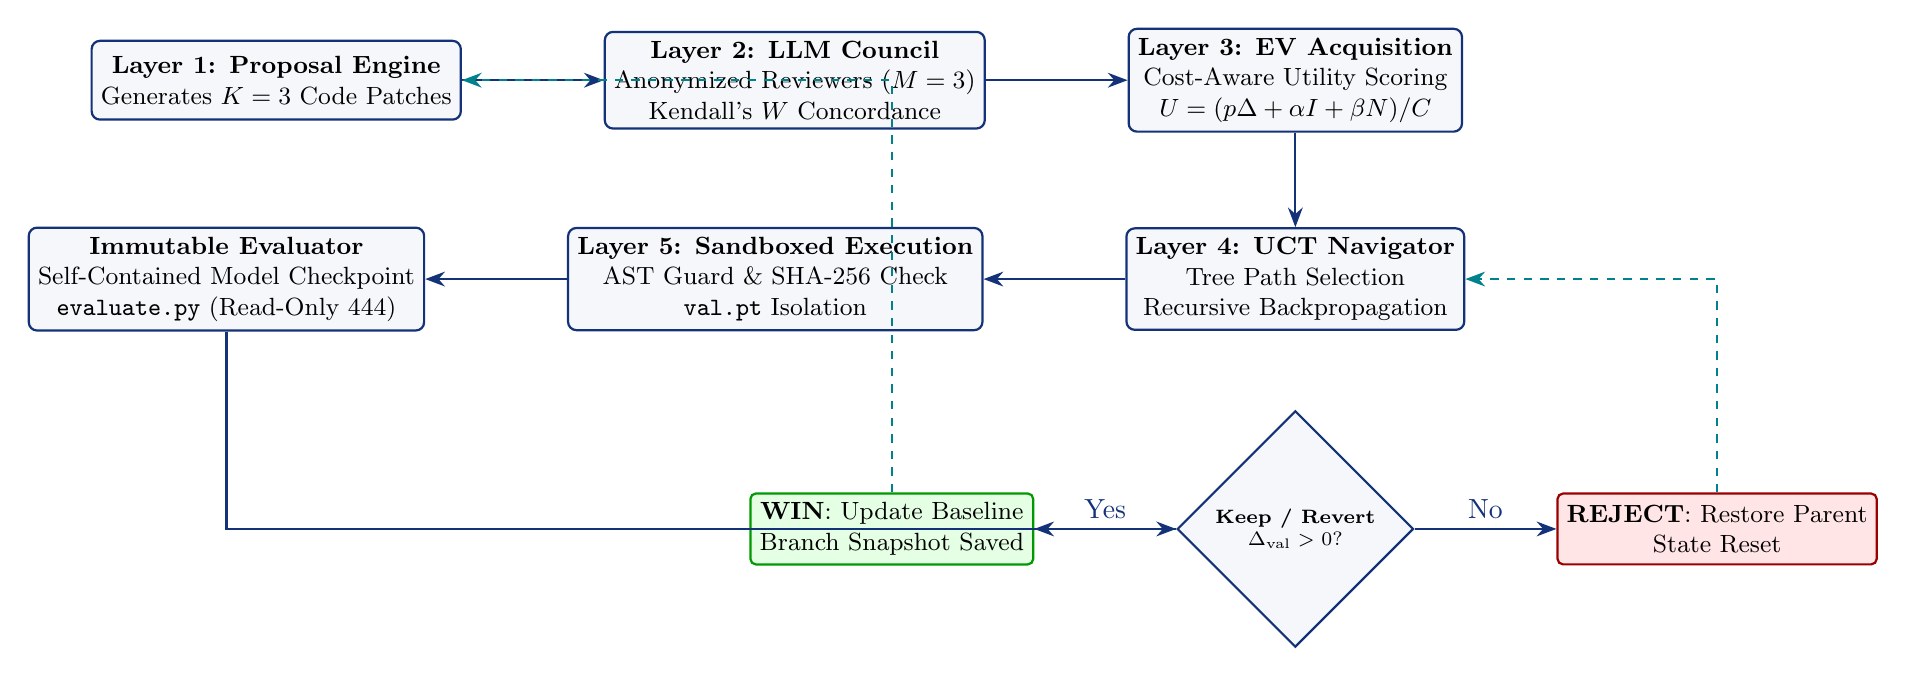
\begin{tikzpicture}[node distance=1.5cm and 1.8cm, auto]
    % Nodes
    \node (proposer) [block] {\textbf{Layer 1: Proposal Engine}\\Generates $K=3$ Code Patches};
    \node (council) [block, right=of proposer] {\textbf{Layer 2: LLM Council}\\Anonymized Reviewers ($M=3$)\\Kendall's $W$ Concordance};
    \node (acquisition) [block, right=of council] {\textbf{Layer 3: EV Acquisition}\\Cost-Aware Utility Scoring\\$U = (p\Delta + \alpha I + \beta N)/C$};
    \node (uct) [block, below=1.2cm of acquisition] {\textbf{Layer 4: UCT Navigator}\\Tree Path Selection\\Recursive Backpropagation};
    \node (sandbox) [block, left=of uct] {\textbf{Layer 5: Sandboxed Execution}\\AST Guard \& SHA-256 Check\\\texttt{val.pt} Isolation};
    \node (evaluator) [block, left=of sandbox] {\textbf{Immutable Evaluator}\\Self-Contained Model Checkpoint\\\texttt{evaluate.py} (Read-Only 444)};
    \node (decision) [decision, below=1.0cm of uct] {\textbf{Keep / Revert}\\$\Delta_{\text{val}} > 0$?};
    \node (win) [process, left=1.8cm of decision, fill=green!10, draw=green!60!black] {\textbf{WIN}: Update Baseline\\Branch Snapshot Saved};
    \node (revert) [process, right=1.8cm of decision, fill=red!10, draw=red!60!black] {\textbf{REJECT}: Restore Parent\\State Reset};

    % Paths
    \draw [line] (proposer) -- (council);
    \draw [line] (council) -- (acquisition);
    \draw [line] (acquisition) -- (uct);
    \draw [line] (uct) -- (sandbox);
    \draw [line] (sandbox) -- (evaluator);
    \draw [line] (evaluator) |- (decision);
    \draw [line] (decision) -- node[above] {Yes} (win);
    \draw [line] (decision) -- node[above] {No} (revert);
    \draw [dashedline] (win) |- (proposer);
    \draw [dashedline] (revert) |- (uct);
\end{tikzpicture}
\caption{System architecture of HypothesisOS depicting the five-layer feedback loop from proposal generation to sandboxed execution, immutable evaluation, and state-tree memory updates.}
\label{fig:tikz_architecture}
\end{figure*}

\subsection{Layer 1: Multi-Hypothesis Proposal Engine}

The Proposal Engine receives the current research plan, synthesized insights from prior wins/failures, and the current \texttt{train.py} code state. It generates $K=3$ mutually exclusive candidate hypotheses represented as unified code diffs.

\subsection{Layer 2: Anonymized Multi-LLM Review Council}

Candidate proposals are presented simultaneously to $M=3$ independent reviewer models (e.g., Llama-3.3-70B, DeepSeek-R1, Gemini-2.5-Flash) with randomized labels ($\text{Proposal A}$, $\text{Proposal B}$, $\text{Proposal C}$).

Reviewers return ordinal rankings and quantitative predictions for expected improvement $\Delta$, success probability $p$, information gain $I$, novelty $N$, and implementation cost $C$.

\subsubsection{Concordance \& Disagreement Modeling}

To measure consensus rigor, we compute Kendall's Coefficient of Concordance $W \in [0.0, 1.0]$ across the reviewer rank matrix $\mathbf{R} \in \mathbb{R}^{M \times K}$:
\begin{equation}
    W = \frac{12 \sum_{j=1}^{K} \left( R_j - \bar{R} \right)^2}{M^2 (K^3 - K)}
    \label{eq:kendalls_w}
\end{equation}
where $R_j$ is the sum of ranks for proposal $j$, and $\bar{R}$ is the mean rank sum. Rank disagreement $D = 1.0 - W$ serves as a dynamic control signal to adjust trial compute allocation:
\begin{equation}
    S_{\text{budget}} = 1.0 + 0.5 \cdot D
    \label{eq:budget_scalar}
\end{equation}

Reviewer ordinal rankings are aggregated using mean-rank scoring $\bar{r}_j = \frac{1}{M} \sum_{i=1}^M R_{ij}$.

\subsection{Layer 3: Cost-Aware Expected-Value Acquisition}

Proposals are ranked according to a multi-attribute utility acquisition function that explicitly balances improvement, surprise, novelty, and compute cost:
\begin{equation}
    U_j = \frac{p_j \cdot \Delta_j + \alpha \cdot I_j + \beta \cdot N_j}{C_j} \cdot \left[ 0.5 + 0.5 \cdot \left( \frac{K - \bar{r}_j + 1}{K} \right) \right]
    \label{eq:ev_acquisition}
\end{equation}
where $\alpha = 0.2$ and $\beta = 0.1$ weight information gain and novelty relative to predicted BPB improvement.

\subsection{Layer 4: State-Tree UCT Search \& Backpropagation}

Rather than conducting greedy selection over flat experiment lists, HypothesisOS organizes experiments as a Directed Acyclic Graph (DAG) state tree.

\begin{figure}[h]
\centering
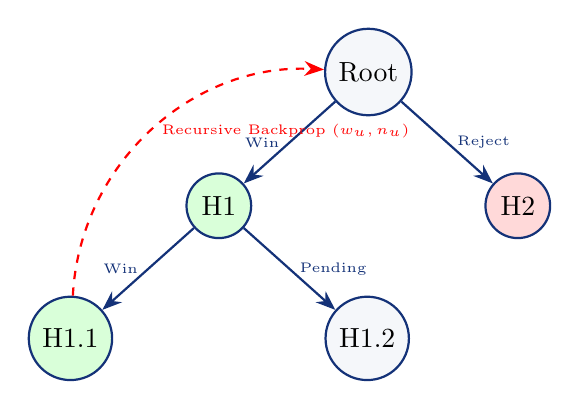
\begin{tikzpicture}[node distance=1.0cm and 1.2cm, auto]
    \node (root) [circle, draw=primaryblue, fill=boxbg, thick] {Root};
    \node (h1) [circle, draw=primaryblue, fill=green!15, thick, below left=of root] {H1};
    \node (h2) [circle, draw=primaryblue, fill=red!15, thick, below right=of root] {H2};
    \node (h11) [circle, draw=primaryblue, fill=green!15, thick, below left=of h1] {H1.1};
    \node (h12) [circle, draw=primaryblue, fill=boxbg, thick, below right=of h1] {H1.2};

    \draw [line] (root) -- node[left, font=\tiny] {Win} (h1);
    \draw [line] (root) -- node[right, font=\tiny] {Reject} (h2);
    \draw [line] (h1) -- node[left, font=\tiny] {Win} (h11);
    \draw [line] (h1) -- node[right, font=\tiny] {Pending} (h12);

    \draw [dashedline, red] (h11) to [bend left=45] node[right, font=\tiny] {Recursive Backprop ($w_u, n_u$)} (root);
\end{tikzpicture}
\caption{UCT State-Tree search structure showing node expansion, branch-isolated state retention, and recursive value backpropagation up to root.}
\label{fig:tikz_uct_tree}
\end{figure}

\subsubsection{Path Traversal via UCT}

Starting at \texttt{root}, the controller traverses child branches by selecting at each node $u$ the child $v$ that maximizes the Upper Confidence bounds applied to Trees (UCT) metric:
\begin{equation}
    \text{UCT}(v) = \frac{w_v}{n_v} + c \cdot \sqrt{\frac{\ln n_{\text{parent}}}{n_v}}
    \label{eq:uct_formula}
\end{equation}
where $w_v$ is total branch wins, $n_v$ is node visit count, and $c = 1.414$ is the exploration parameter.

\subsubsection{Recursive Value Backpropagation}

Upon trial completion, outcome $w_{\text{trial}} \in \{0, 1\}$ is recursively backpropagated from the leaf node along all parent pointers up to \texttt{root}:
\begin{equation}
    \forall u \in \text{Path}(\text{leaf} \to \text{root}): \quad n_u \leftarrow n_u + 1, \quad w_u \leftarrow w_u + \mathbb{I}(\text{win})
\end{equation}

\subsubsection{Branch-Isolated State Restoration}

To guarantee exact state isolation, every node stores \texttt{full\_code\_snapshot}. When expanding branch $P$, \texttt{orchestrator.py} explicitly restores $P$'s source code snapshot to \texttt{train.py} before applying new candidate diffs, preventing cross-branch state contamination.

\subsection{Layer 5: Sandboxed Execution \& Immutable Evaluation Boundary}

To safeguard against evaluator tampering and data leakage:
\begin{enumerate}
    \item \textbf{Self-Contained Evaluator}: \texttt{evaluate.py} imports zero modules from \texttt{train.py} and reconstructs its model architecture directly from \texttt{model.pt} checkpoint metadata.
    \item \textbf{SHA-256 Hash Verification}: At startup, \texttt{orchestrator.py} computes the SHA-256 digest of \texttt{evaluate.py} and locks the file to read-only permissions (\texttt{chmod 444}). Integrity is re-verified prior to every evaluation run.
    \item \textbf{Validation Data Isolation}: Security guards explicitly reject any candidate code patch containing references to \texttt{data/val.pt} or direct metric manipulation (\texttt{val\_bpb}).
    \item \textbf{RNG Decoupling}: Independent PyTorch \texttt{Generator} instances (\texttt{BATCH\_RNG}) isolate dataset batch sampling from neural network initialization seeds.
\end{enumerate}

\section{Experimental Protocol}
\label{sec:experiments}

To evaluate whether cost-aware multi-agent control yields statistically significant gains in compute efficiency, we formulate a 7-armed factorial ablation study.

\subsection{Ablation Arms}
\begin{enumerate}
    \item \textbf{Arm A (Single-Agent AutoResearch)}: Single LLM propose-and-execute loop (Karpathy baseline).
    \item \textbf{Arm B (Random Search)}: Uniformly random hyperparameter/architecture perturbations.
    \item \textbf{Arm C (Single-LLM Direct Choice)}: Multi-proposal generation with single-agent greedy selection.
    \item \textbf{Arm D (Mean-Rank Council)}: Anonymized multi-LLM review with mean-rank scoring (no cost term).
    \item \textbf{Arm E (Council + Memory)}: Anonymized council with persistent failure memory.
    \item \textbf{Arm F (Council + Memory + UCT)}: Council review with state-tree UCT search expansion.
    \item \textbf{Arm G (Full Cost-Aware EV Controller)}: Full HypothesisOS framework utilizing Eq.~(\ref{eq:ev_acquisition}) with disagreement compute scaling.
\end{enumerate}

\subsection{Evaluation Tasks \& Statistical Criteria}

Experiments will be conducted across two standardized benchmarks under fixed wall-clock GPU budgets:
\begin{itemize}
    \item \textbf{Task 1 (TinyShakespeare)}: Character-level LM (~1.1M chars), 30-second compute budget per trial, 3-hour allocation ($R=10$ replicates).
    \item \textbf{Task 2 (WikiText-103)}: Word-level LM (~100M tokens), 15-minute compute budget per trial, 12-hour allocation ($R=5$ replicates).
\end{itemize}

Statistical significance will be established using paired $t$-tests and Wilcoxon signed-rank tests ($\alpha = 0.05$), reporting Cohen's $d$ effect sizes and 95\% bootstrap confidence intervals.

\section{Risk Analysis \& Mitigations}
\label{sec:risks}

Table~\ref{tab:risks} details key system failure modes and mitigation mechanisms implemented in HypothesisOS.

\begin{table}[h]
\centering
\caption{System risk analysis and mitigation protocols.}
\label{tab:risks}
\small
\resizebox{\linewidth}{!}{%
\begin{tabular}{l l}
\toprule
\textbf{Identified Risk Mode} & \textbf{Engineered Mitigation Protocol} \\
\midrule
Evaluator Tampering & SHA-256 hash lock + \texttt{chmod 444} read-only guard. \\
Validation Data Leakage & Static AST filter blocking \texttt{data/val.pt} access. \\
LLM Miscalibration & Isotonic calibration over historical proposal logs. \\
Greedy Search Collapse & State-tree UCT path expansion with $c=1.414$. \\
Cross-Branch Leakage & Snapshot code restoration (\texttt{full\_code\_snapshot}). \\
\bottomrule
\end{tabular}%
}
\end{table}

\section{Implementation Roadmap}
\label{sec:roadmap}

The research lifecycle is structured into eight phases requiring approximately 600 GPU hours and $5 \times 10^5$ LLM API tokens (Table~\ref{tab:roadmap}).

\begin{table}[h]
\centering
\caption{Phased development roadmap and resource allocation.}
\label{tab:roadmap}
\small
\resizebox{\linewidth}{!}{%
\begin{tabular}{l c l}
\toprule
\textbf{Phase / Milestone} & \textbf{Duration} & \textbf{Primary Output} \\
\midrule
1. Architecture Design & 2 Weeks & Formal System Specification \\
2. Infrastructure Setup & 2 Weeks & Isolated Execution Sandbox \\
3. Council \& UCT Core & 3 Weeks & Multi-Model Concordance Engine \\
4. Calibration Module & 2 Weeks & Isotonic EV Calibration \\
5. Small Benchmark Runs & 4 Weeks & TinyShakespeare Ablation Data \\
6. Scaling Benchmark & 4 Weeks & WikiText-103 Empirical Results \\
7. Statistical Synthesis & 2 Weeks & Effect Size \& CI Analysis \\
8. Publication & 2 Weeks & Camera-Ready Paper Submission \\
\bottomrule
\end{tabular}%
}
\end{table}

\section{Conclusion}
\label{sec:conclusion}

HypothesisOS advances autonomous machine learning by shifting focus from unconstrained code generation to compute-normalized experiment control. By combining anonymized multi-LLM deliberation, cost-aware expected-value acquisition, state-tree UCT search with recursive backpropagation, and strict sandboxed evaluation boundaries, HypothesisOS establishes a rigorous foundation for reproducible, cost-efficient AI scientific discovery.

% --- References ---
\begin{thebibliography}{99}

\bibitem{karpathy2026autoresearch}
A.~Karpathy, ``AutoResearch: Autonomous single-agent machine learning optimization loop,'' \textit{GitHub Repository}, Mar. 2026.

\bibitem{karpathy2025llmcouncil}
A.~Karpathy, ``LLM Council: Anonymized multi-agent peer review and rank aggregation,'' \textit{Technical Report}, Nov. 2025.

\bibitem{lu2024aiscientist}
C.~Lu, C.~Lu, R.~Lange, S.~Foerster, and D.~Ha, ``The AI Scientist: Towards fully automated open-ended scientific discovery,'' \textit{arXiv preprint arXiv:2408.06292}, Aug. 2024.

\bibitem{lu2025aiscientistv2}
C.~Lu, C.~Lu, and D.~Ha, ``The AI Scientist v2: Progressive agentic tree search for autonomous machine learning research,'' \textit{arXiv preprint arXiv:2504.08066}, Apr. 2025; \textit{Nature}, 2026.

\bibitem{lu2026evoscientist}
Y.~Lu et al., ``EvoScientist: Towards multi-agent evolving AI scientists for end-to-end scientific discovery,'' \textit{arXiv preprint arXiv:2603.08127}, Mar. 2026.

\bibitem{autodiscovery2025}
Anonymous, ``AutoDiscovery: Open-ended scientific hypothesis search via Bayesian surprise MCTS,'' in \textit{Proc. Advances in Neural Information Processing Systems (NeurIPS)}, Dec. 2025.

\bibitem{consensusnas2026}
Anonymous, ``Consensus-gated multi-agent neural architecture search,'' \textit{arXiv preprint arXiv:2608.13889}, Aug. 2026.

\bibitem{alphaevolve2025}
Google DeepMind, ``AlphaEvolve: Evolutionary LLM discovery of matrix multiplication algorithms,'' \textit{Technical Report}, Jun. 2025.

\end{thebibliography}

\end{document}
